\section{Neural network implementation}
A {\it mhcflurry} predictor consists of a embedding layer which transforms each amino acid to a learned vector representation, followed by a single hidden layer and finally a scalar output (figure \ref{architecture}). We map IC50 concentrations onto a regression target between 0.0 and 1.0 using the same scheme as NetMHC, $y = 1.0 - max(1.0, log_{50000}(IC50))$.

\begin{figure}[h]
\centering
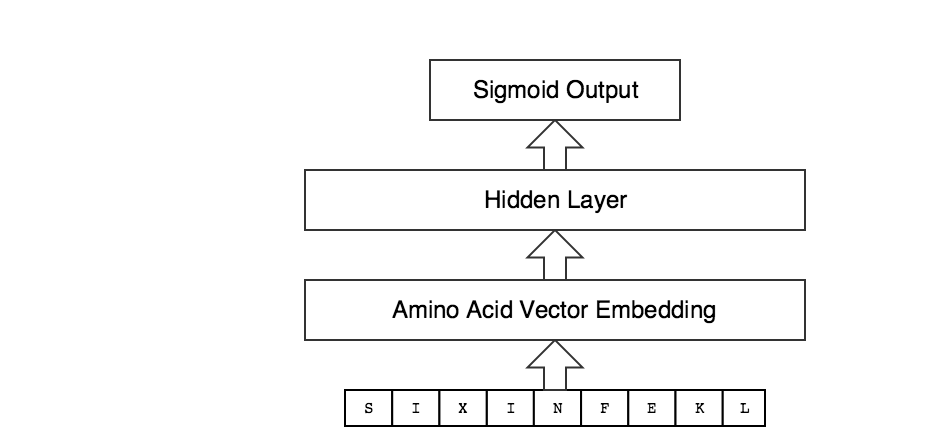
\includegraphics[scale=0.5]{figures/mhcflurry-gliffy-network.png}
\caption{Neural network architecture for predicting peptide-MHC affinities from fixed length amino acid sequences}
\label{fig:architecture}
\end{figure}

Like NetMHC\cite{lundegaard2008accurate}, the mhcflurry predictor assumes length-9 peptides and uses an averaging scheme to reduce non-9mer peptides to a 9mer prediction task. Briefly, each non-9mer is mapped into multiple 9mer query peptides by introducing a sentinel ``X'' at every position or removing consecutive stretches of residues, and the predicted affinity is taken to be the geometric mean of the predictions for the queries. This scheme is also used for training.

For each allele, we train a mhcflurry model using the measured peptide affinities for the allele and the values imputed by MICE based on other alleles in the training set. As training progresses, we place decreasing weight on the imputed values. Each imputed value's weight at training epoch $i$ is set to $1 / (1 + i)^2$.

A randomly generated peptide is unlikely to bind a given MHC strongly, but a data acquisition bias toward strong binders in the training set can lead models to erroneously assign most peptides high affinity. As a form of regularization, we augment the training set at each epoch to include random peptides with affinity set to be maximally weak. The peptides are generated by drawing amino acids uniformly at random. The number of random negative peptides is 20\% of the training size (without imputation). At each training epoch, a fresh set of random peptides is generated.

Three-fold cross validation on the training set was used to select the hyper-parameters. The model selected used 32 output dimensions for the amino acid vector embedding, a hidden layer size of 64, a dropout rate\cite{Srivastava2014} of 50\%, and 250 training epochs. These hyper-parameters achieved reasonable performance across alleles, but it's likely that performance could be slightly improved by setting the hyper-parameters separately for each allele.